\chapter{Chapter VIII}

\begin{verse}
At this the challenger with fierce defy\\
His trumpet sounds; the challenged makes reply:\\
With clangour rings the field, resounds the vaulted sky.\\
Their visors closed, their lances in the rest,\\
Or at the helmet pointed or the crest,\\
They vanish from the barrier, speed the race,\\
And spurring see decrease the middle space.\\!
\attrib{Palamon and Arcite}
\end{verse}

\lettrine{I}{n} the midst of Prince John's cavalcade, he suddenly stopt, and
appealing to the Prior of Jorvaulx, declared the principal business of
the day had been forgotten.

``By my halidom,'' said he, ``we have forgotten, Sir Prior, to name the
fair Sovereign of Love and of Beauty, by whose white hand the palm is to
be distributed. For my part, I am liberal in my ideas, and I care not if
I give my vote for the black-eyed Rebecca.''

``Holy Virgin,'' answered the Prior, turning up his eyes in horror, ``a
Jewess!--We should deserve to be stoned out of the lists; and I am not
yet old enough to be a martyr. Besides, I swear by my patron saint, that
she is far inferior to the lovely Saxon, Rowena.''

``Saxon or Jew,'' answered the Prince, ``Saxon or Jew, dog or hog, what
matters it? I say, name Rebecca, were it only to mortify the Saxon
churls.''

A murmur arose even among his own immediate attendants.

``This passes a jest, my lord,'' said De Bracy; ``no knight here will
lay lance in rest if such an insult is attempted.''

``It is the mere wantonness of insult,'' said one of the oldest and most
important of Prince John's followers, Waldemar Fitzurse, ``and if your
Grace attempt it, cannot but prove ruinous to your projects.''

``I entertained you, sir,'' said John, reining up his palfrey haughtily,
``for my follower, but not for my counsellor.''

``Those who follow your Grace in the paths which you tread,'' said
Waldemar, but speaking in a low voice, ``acquire the right of
counsellors; for your interest and safety are not more deeply gaged than
their own.''

From the tone in which this was spoken, John saw the necessity of
acquiescence ``I did but jest,'' he said; ``and you turn upon me like so
many adders! Name whom you will, in the fiend's name, and please
yourselves.''

``Nay, nay,'' said De Bracy, ``let the fair sovereign's throne remain
unoccupied, until the conqueror shall be named, and then let him choose
the lady by whom it shall be filled. It will add another grace to his
triumph, and teach fair ladies to prize the love of valiant knights, who
can exalt them to such distinction.''

``If Brian de Bois-Guilbert gain the prize,'' said the Prior, ``I will
gage my rosary that I name the Sovereign of Love and Beauty.''

``Bois-Guilbert,'' answered De Bracy, ``is a good lance; but there are
others around these lists, Sir Prior, who will not fear to encounter
him.''

``Silence, sirs,'' said Waldemar, ``and let the Prince assume his seat.
The knights and spectators are alike impatient, the time advances, and
highly fit it is that the sports should commence.''

Prince John, though not yet a monarch, had in Waldemar Fitzurse all the
inconveniences of a favourite minister, who, in serving his sovereign,
must always do so in his own way. The Prince acquiesced, however,
although his disposition was precisely of that kind which is apt to be
obstinate upon trifles, and, assuming his throne, and being surrounded
by his followers, gave signal to the heralds to proclaim the laws of the
tournament, which were briefly as follows:

First, the five challengers were to undertake all comers.

Secondly, any knight proposing to combat, might, if he pleased, select a
special antagonist from among the challengers, by touching his shield.
If he did so with the reverse of his lance, the trial of skill was made
with what were called the arms of courtesy, that is, with lances at
whose extremity a piece of round flat board was fixed, so that no danger
was encountered, save from the shock of the horses and riders. But if
the shield was touched with the sharp end of the lance, the combat was
understood to be at ``outrance'', that is, the knights were to fight
with sharp weapons, as in actual battle.

Thirdly, when the knights present had accomplished their vow, by each of
them breaking five lances, the Prince was to declare the victor in the
first day's tourney, who should receive as prize a warhorse of exquisite
beauty and matchless strength; and in addition to this reward of valour,
it was now declared, he should have the peculiar honour of naming the
Queen of Love and Beauty, by whom the prize should be given on the
ensuing day.

Fourthly, it was announced, that, on the second day, there should be a
general tournament, in which all the knights present, who were desirous
to win praise, might take part; and being divided into two bands of
equal numbers, might fight it out manfully, until the signal was given
by Prince John to cease the combat. The elected Queen of Love and Beauty
was then to crown the knight whom the Prince should adjudge to have
borne himself best in this second day, with a coronet composed of thin
gold plate, cut into the shape of a laurel crown. On this second day the
knightly games ceased. But on that which was to follow, feats of
archery, of bull-baiting, and other popular amusements, were to be
practised, for the more immediate amusement of the populace. In this
manner did Prince John endeavour to lay the foundation of a popularity,
which he was perpetually throwing down by some inconsiderate act of
wanton aggression upon the feelings and prejudices of the people.

The lists now presented a most splendid spectacle. The sloping galleries
were crowded with all that was noble, great, wealthy, and beautiful in
the northern and midland parts of England; and the contrast of the
various dresses of these dignified spectators, rendered the view as gay
as it was rich, while the interior and lower space, filled with the
substantial burgesses and yeomen of merry England, formed, in their more
plain attire, a dark fringe, or border, around this circle of brilliant
embroidery, relieving, and, at the same time, setting off its splendour.

The heralds finished their proclamation with their usual cry of
``Largesse, largesse, gallant knights!'' and gold and silver pieces were
showered on them from the galleries, it being a high point of chivalry
to exhibit liberality towards those whom the age accounted at once the
secretaries and the historians of honour. The bounty of the spectators
was acknowledged by the customary shouts of ``Love of Ladies--Death of
Champions--Honour to the Generous--Glory to the Brave!'' To which the
more humble spectators added their acclamations, and a numerous band of
trumpeters the flourish of their martial instruments. When these sounds
had ceased, the heralds withdrew from the lists in gay and glittering
procession, and none remained within them save the marshals of the
field, who, armed cap-a-pie, sat on horseback, motionless as statues, at
the opposite ends of the lists. Meantime, the enclosed space at the
northern extremity of the lists, large as it was, was now completely
crowded with knights desirous to prove their skill against the
challengers, and, when viewed from the galleries, presented the
appearance of a sea of waving plumage, intermixed with glistening
helmets, and tall lances, to the extremities of which were, in many
cases, attached small pennons of about a span's breadth, which,
fluttering in the air as the breeze caught them, joined with the
restless motion of the feathers to add liveliness to the scene.

At length the barriers were opened, and five knights, chosen by lot,
advanced slowly into the area; a single champion riding in front, and
the other four following in pairs. All were splendidly armed, and my
Saxon authority (in the Wardour Manuscript) records at great length
their devices, their colours, and the embroidery of their horse
trappings. It is unnecessary to be particular on these subjects. To
borrow lines from a contemporary poet, who has written but too little:

\begin{verse}
``The knights are dust,\\
And their good swords are rust,\\
Their souls are with the saints, we trust.''\footnote{These lines are
part of an unpublished poem, by
Coleridge, whose Muse so often tantalizes with fragments which indicate
her powers, while the manner in which she flings them from her betrays
her caprice, yet whose unfinished sketches display more talent than the
laboured masterpieces of others.}\\!
\end{verse}

Their escutcheons have long mouldered from the walls of their castles.
Their castles themselves are but green mounds and shattered ruins--the
place that once knew them, knows them no more--nay, many a race since
theirs has died out and been forgotten in the very land which they
occupied, with all the authority of feudal proprietors and feudal lords.
What, then, would it avail the reader to know their names, or the
evanescent symbols of their martial rank!

Now, however, no whit anticipating the oblivion which awaited their
names and feats, the champions advanced through the lists, restraining
their fiery steeds, and compelling them to move slowly, while, at the
same time, they exhibited their paces, together with the grace and
dexterity of the riders. As the procession entered the lists, the sound
of a wild Barbaric music was heard from behind the tents of the
challengers, where the performers were concealed. It was of Eastern
origin, having been brought from the Holy Land; and the mixture of the
cymbals and bells seemed to bid welcome at once, and defiance, to the
knights as they advanced. With the eyes of an immense concourse of
spectators fixed upon them, the five knights advanced up the platform
upon which the tents of the challengers stood, and there separating
themselves, each touched slightly, and with the reverse of his lance,
the shield of the antagonist to whom he wished to oppose himself. The
lower orders of spectators in general--nay, many of the higher class,
and it is even said several of the ladies, were rather disappointed at
the champions choosing the arms of courtesy. For the same sort of
persons, who, in the present day, applaud most highly the deepest
tragedies, were then interested in a tournament exactly in proportion to
the danger incurred by the champions engaged.

Having intimated their more pacific purpose, the champions retreated to
the extremity of the lists, where they remained drawn up in a line;
while the challengers, sallying each from his pavilion, mounted their
horses, and, headed by Brian de Bois-Guilbert, descended from the
platform, and opposed themselves individually to the knights who had
touched their respective shields.

At the flourish of clarions and trumpets, they started out against each
other at full gallop; and such was the superior dexterity or good
fortune of the challengers, that those opposed to Bois-Guilbert,
Malvoisin, and Front-de-Boeuf, rolled on the ground. The antagonist of
Grantmesnil, instead of bearing his lance-point fair against the crest
or the shield of his enemy, swerved so much from the direct line as to
break the weapon athwart the person of his opponent--a circumstance
which was accounted more disgraceful than that of being actually
unhorsed; because the latter might happen from accident, whereas the
former evinced awkwardness and want of management of the weapon and of
the horse. The fifth knight alone maintained the honour of his party,
and parted fairly with the Knight of St John, both splintering their
lances without advantage on either side.

The shouts of the multitude, together with the acclamations of the
heralds, and the clangour of the trumpets, announced the triumph of the
victors and the defeat of the vanquished. The former retreated to their
pavilions, and the latter, gathering themselves up as they could,
withdrew from the lists in disgrace and dejection, to agree with their
victors concerning the redemption of their arms and their horses, which,
according to the laws of the tournament, they had forfeited. The fifth
of their number alone tarried in the lists long enough to be greeted by
the applauses of the spectators, amongst whom he retreated, to the
aggravation, doubtless, of his companions' mortification.

A second and a third party of knights took the field; and although they
had various success, yet, upon the whole, the advantage decidedly
remained with the challengers, not one of whom lost his seat or swerved
from his charge--misfortunes which befell one or two of their
antagonists in each encounter. The spirits, therefore, of those opposed
to them, seemed to be considerably damped by their continued success.
Three knights only appeared on the fourth entry, who, avoiding the
shields of Bois-Guilbert and Front-de-Boeuf, contented themselves with
touching those of the three other knights, who had not altogether
manifested the same strength and dexterity. This politic selection did
not alter the fortune of the field, the challengers were still
successful: one of their antagonists was overthrown, and both the others
failed in the ``attaint'',\footnote{This term of chivalry, transferred to
the law, gives the
phrase of being attainted of treason.} that is, in striking the helmet and
shield of their antagonist firmly and strongly, with the lance held in a
direct line, so that the weapon might break unless the champion was
overthrown.

After this fourth encounter, there was a considerable pause; nor did it
appear that any one was very desirous of renewing the contest. The
spectators murmured among themselves; for, among the challengers,
Malvoisin and Front-de-Boeuf were unpopular from their characters, and
the others, except Grantmesnil, were disliked as strangers and
foreigners.

But none shared the general feeling of dissatisfaction so keenly as
Cedric the Saxon, who saw, in each advantage gained by the Norman
challengers, a repeated triumph over the honour of England. His own
education had taught him no skill in the games of chivalry, although,
with the arms of his Saxon ancestors, he had manifested himself, on many
occasions, a brave and determined soldier. He looked anxiously to
Athelstane, who had learned the accomplishments of the age, as if
desiring that he should make some personal effort to recover the victory
which was passing into the hands of the Templar and his associates. But,
though both stout of heart, and strong of person, Athelstane had a
disposition too inert and unambitious to make the exertions which Cedric
seemed to expect from him.

``The day is against England, my lord,'' said Cedric, in a marked tone;
``are you not tempted to take the lance?''

``I shall tilt to-morrow'' answered Athelstane, ``in the `melee'; it is
not worth while for me to arm myself to-day.''

Two things displeased Cedric in this speech. It contained the Norman
word ``melee'', (to express the general conflict,) and it evinced some
indifference to the honour of the country; but it was spoken by
Athelstane, whom he held in such profound respect, that he would not
trust himself to canvass his motives or his foibles. Moreover, he had no
time to make any remark, for Wamba thrust in his word, observing, ``It
was better, though scarce easier, to be the best man among a hundred,
than the best man of two.''

Athelstane took the observation as a serious compliment; but Cedric, who
better understood the Jester's meaning, darted at him a severe and
menacing look; and lucky it was for Wamba, perhaps, that the time and
place prevented his receiving, notwithstanding his place and service,
more sensible marks of his master's resentment.

The pause in the tournament was still uninterrupted, excepting by the
voices of the heralds exclaiming--``Love of ladies, splintering of
lances! stand forth gallant knights, fair eyes look upon your deeds!''

The music also of the challengers breathed from time to time wild bursts
expressive of triumph or defiance, while the clowns grudged a holiday
which seemed to pass away in inactivity; and old knights and nobles
lamented in whispers the decay of martial spirit, spoke of the triumphs
of their younger days, but agreed that the land did not now supply dames
of such transcendent beauty as had animated the jousts of former times.
Prince John began to talk to his attendants about making ready the
banquet, and the necessity of adjudging the prize to Brian de
Bois-Guilbert, who had, with a single spear, overthrown two knights, and
foiled a third.

At length, as the Saracenic music of the challengers concluded one of
those long and high flourishes with which they had broken the silence of
the lists, it was answered by a solitary trumpet, which breathed a note
of defiance from the northern extremity. All eyes were turned to see the
new champion which these sounds announced, and no sooner were the
barriers opened than he paced into the lists. As far as could be judged
of a man sheathed in armour, the new adventurer did not greatly exceed
the middle size, and seemed to be rather slender than strongly made. His
suit of armour was formed of steel, richly inlaid with gold, and the
device on his shield was a young oak-tree pulled up by the roots, with
the Spanish word Desdichado, signifying Disinherited. He was mounted on
a gallant black horse, and as he passed through the lists he gracefully
saluted the Prince and the ladies by lowering his lance. The dexterity
with which he managed his steed, and something of youthful grace which
he displayed in his manner, won him the favour of the multitude, which
some of the lower classes expressed by calling out, ``Touch Ralph de
Vipont's shield--touch the Hospitallers shield; he has the least sure
seat, he is your cheapest bargain.''

The champion, moving onward amid these well-meant hints, ascended the
platform by the sloping alley which led to it from the lists, and, to
the astonishment of all present, riding straight up to the central
pavilion, struck with the sharp end of his spear the shield of Brian de
Bois-Guilbert until it rung again. All stood astonished at his
presumption, but none more than the redoubted Knight whom he had thus
defied to mortal combat, and who, little expecting so rude a challenge,
was standing carelessly at the door of the pavilion.

``Have you confessed yourself, brother,'' said the Templar, ``and have
you heard mass this morning, that you peril your life so frankly?''

``I am fitter to meet death than thou art'' answered the Disinherited
Knight; for by this name the stranger had recorded himself in the books
of the tourney.

``Then take your place in the lists,'' said Bois-Guilbert, ``and look
your last upon the sun; for this night thou shalt sleep in paradise.''

``Gramercy for thy courtesy,'' replied the Disinherited Knight, ``and to
requite it, I advise thee to take a fresh horse and a new lance, for by
my honour you will need both.''

Having expressed himself thus confidently, he reined his horse backward
down the slope which he had ascended, and compelled him in the same
manner to move backward through the lists, till he reached the northern
extremity, where he remained stationary, in expectation of his
antagonist. This feat of horsemanship again attracted the applause of
the multitude.

However incensed at his adversary for the precautions which he
recommended, Brian de Bois-Guilbert did not neglect his advice; for his
honour was too nearly concerned, to permit his neglecting any means
which might ensure victory over his presumptuous opponent. He changed
his horse for a proved and fresh one of great strength and spirit. He
chose a new and a tough spear, lest the wood of the former might have
been strained in the previous encounters he had sustained. Lastly, he
laid aside his shield, which had received some little damage, and
received another from his squires. His first had only borne the general
device of his rider, representing two knights riding upon one horse, an
emblem expressive of the original humility and poverty of the Templars,
qualities which they had since exchanged for the arrogance and wealth
that finally occasioned their suppression. Bois-Guilbert's new shield
bore a raven in full flight, holding in its claws a skull, and bearing
the motto, ``Gare le Corbeau''.

When the two champions stood opposed to each other at the two
extremities of the lists, the public expectation was strained to the
highest pitch. Few augured the possibility that the encounter could
terminate well for the Disinherited Knight, yet his courage and
gallantry secured the general good wishes of the spectators.

The trumpets had no sooner given the signal, than the champions vanished
from their posts with the speed of lightning, and closed in the centre
of the lists with the shock of a thunderbolt. The lances burst into
shivers up to the very grasp, and it seemed at the moment that both
knights had fallen, for the shock had made each horse recoil backwards
upon its haunches. The address of the riders recovered their steeds by
use of the bridle and spur; and having glared on each other for an
instant with eyes which seemed to flash fire through the bars of their
visors, each made a demi-volte, and, retiring to the extremity of the
lists, received a fresh lance from the attendants.

A loud shout from the spectators, waving of scarfs and handkerchiefs,
and general acclamations, attested the interest taken by the spectators
in this encounter; the most equal, as well as the best performed, which
had graced the day. But no sooner had the knights resumed their station,
than the clamour of applause was hushed into a silence, so deep and so
dead, that it seemed the multitude were afraid even to breathe.

A few minutes pause having been allowed, that the combatants and their
horses might recover breath, Prince John with his truncheon signed to
the trumpets to sound the onset. The champions a second time sprung from
their stations, and closed in the centre of the lists, with the same
speed, the same dexterity, the same violence, but not the same equal
fortune as before.

In this second encounter, the Templar aimed at the centre of his
antagonist's shield, and struck it so fair and forcibly, that his spear
went to shivers, and the Disinherited Knight reeled in his saddle. On
the other hand, that champion had, in the beginning of his career,
directed the point of his lance towards Bois-Guilbert's shield, but,
changing his aim almost in the moment of encounter, he addressed it to
the helmet, a mark more difficult to hit, but which, if attained,
rendered the shock more irresistible. Fair and true he hit the Norman on
the visor, where his lance's point kept hold of the bars. Yet, even at
this disadvantage, the Templar sustained his high reputation; and had
not the girths of his saddle burst, he might not have been unhorsed. As
it chanced, however, saddle, horse, and man, rolled on the ground under
a cloud of dust.

\begin{figure}
    \centering
    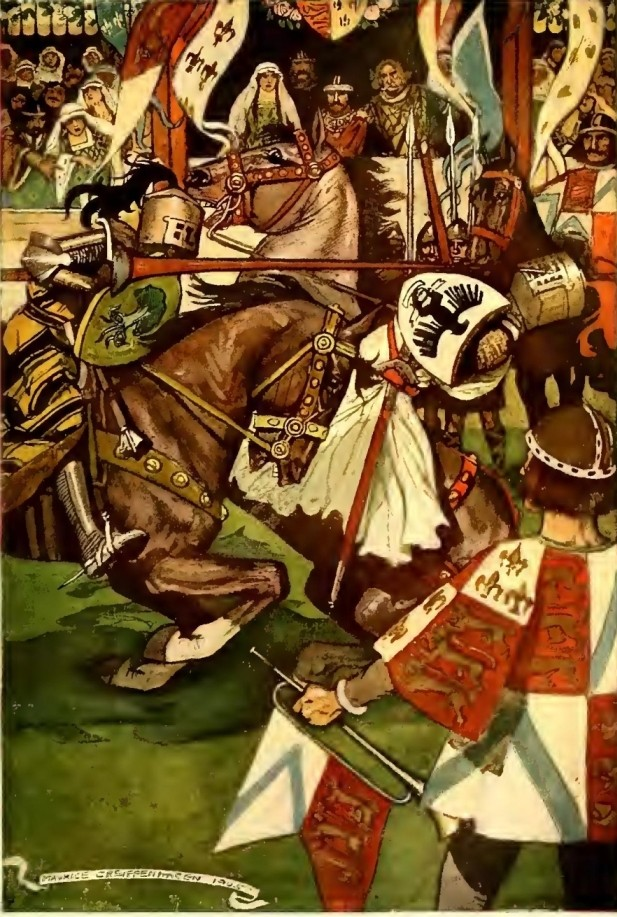
\includegraphics[height=.9\textheight]{ivanhoe/0135m}
    \caption{Fair and true he hit the Norman on the visor.}
\end{figure}

To extricate himself from the stirrups and fallen steed, was to the
Templar scarce the work of a moment; and, stung with madness, both at
his disgrace and at the acclamations with which it was hailed by the
spectators, he drew his sword and waved it in defiance of his conqueror.
The Disinherited Knight sprung from his steed, and also unsheathed his
sword. The marshals of the field, however, spurred their horses between
them, and reminded them, that the laws of the tournament did not, on the
present occasion, permit this species of encounter.

``We shall meet again, I trust,'' said the Templar, casting a resentful
glance at his antagonist; ``and where there are none to separate us.''

``If we do not,'' said the Disinherited Knight, ``the fault shall not be
mine. On foot or horseback, with spear, with axe, or with sword, I am
alike ready to encounter thee.''

More and angrier words would have been exchanged, but the marshals,
crossing their lances betwixt them, compelled them to separate. The
Disinherited Knight returned to his first station, and Bois-Guilbert to
his tent, where he remained for the rest of the day in an agony of
despair.

Without alighting from his horse, the conqueror called for a bowl of
wine, and opening the beaver, or lower part of his helmet, announced
that he quaffed it, ``To all true English hearts, and to the confusion
of foreign tyrants.'' He then commanded his trumpet to sound a defiance
to the challengers, and desired a herald to announce to them, that he
should make no election, but was willing to encounter them in the order
in which they pleased to advance against him.

The gigantic Front-de-Boeuf, armed in sable armour, was the first who
took the field. He bore on a white shield a black bull's head, half
defaced by the numerous encounters which he had undergone, and bearing
the arrogant motto, ``Cave, Adsum''. Over this champion the Disinherited
Knight obtained a slight but decisive advantage. Both Knights broke
their lances fairly, but Front-de-Boeuf, who lost a stirrup in the
encounter, was adjudged to have the disadvantage.

In the stranger's third encounter with Sir Philip Malvoisin, he was
equally successful; striking that baron so forcibly on the casque, that
the laces of the helmet broke, and Malvoisin, only saved from falling by
being unhelmeted, was declared vanquished like his companions.

In his fourth combat with De Grantmesnil, the Disinherited Knight showed
as much courtesy as he had hitherto evinced courage and dexterity. De
Grantmesnil's horse, which was young and violent, reared and plunged in
the course of the career so as to disturb the rider's aim, and the
stranger, declining to take the advantage which this accident afforded
him, raised his lance, and passing his antagonist without touching him,
wheeled his horse and rode back again to his own end of the lists,
offering his antagonist, by a herald, the chance of a second encounter.
This De Grantmesnil declined, avowing himself vanquished as much by the
courtesy as by the address of his opponent.

Ralph de Vipont summed up the list of the stranger's triumphs, being
hurled to the ground with such force, that the blood gushed from his
nose and his mouth, and he was borne senseless from the lists.

The acclamations of thousands applauded the unanimous award of the
Prince and marshals, announcing that day's honours to the Disinherited
Knight.
